\documentclass[tikz, border=15pt]{standalone}
\usepackage{amsmath}
\usetikzlibrary{calc, arrows.meta}

\begin{document}

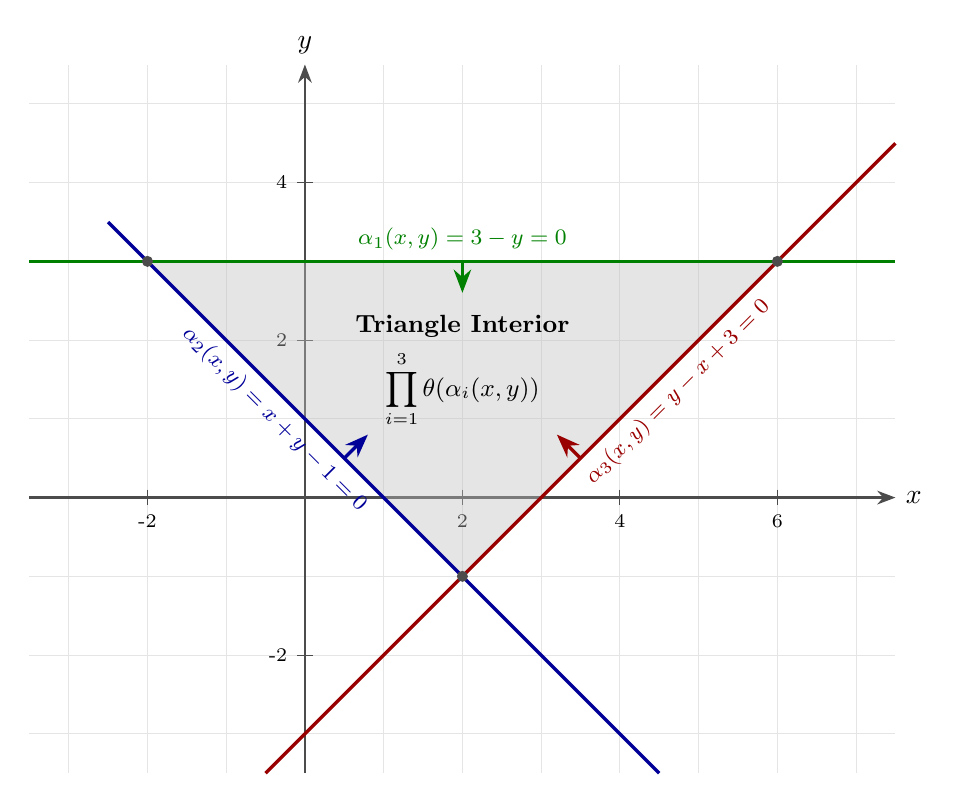
\begin{tikzpicture}[x=1cm, y=1cm, >=Stealth]

    % ==========================================
    % 1. GRID & AXES (Softened to reduce clutter)
    % ==========================================
    % Light grid
    \draw[step=1cm, gray!20, thin] (-3.5, -3.5) grid (7.5, 5.5);

    % Axes
    \draw[->, thick, gray!60!black] (-3.5, 0) -- (7.5, 0) node[right, text=black] {$x$};
    \draw[->, thick, gray!60!black] (0, -3.5) -- (0, 5.5) node[above, text=black] {$y$};
    
    % Axis ticks
    \foreach \x in {-2, 2, 4, 6} {
        \draw[gray!60!black] (\x, 0.1) -- (\x, -0.1) node[below, font=\scriptsize, text=black] {\x};
    }
    \foreach \y in {-2, 2, 4} {
        \draw[gray!60!black] (0.1, \y) -- (-0.1, \y) node[left, font=\scriptsize, text=black] {\y};
    }

    % ==========================================
    % 2. TRIANGLE INTERIOR (Translucent fill)
    % ==========================================
    % Fill only the valid region where all Heaviside functions are 1
    % Made translucent so the grid shows through!
    \fill[gray!50, fill opacity=0.4] (-2, 3) -- (6, 3) -- (2, -1) -- cycle;

    % ==========================================
    % 3. EDGE LINES
    % ==========================================
    % Edge 1 (Top / Green) - Moved to y = 3
    \draw[green!50!black, very thick] (-3.5, 3) -- (7.5, 3) 
        node[pos=0.5, above, font=\footnotesize] {$\alpha_1(x,y) = 3 - y = 0$};
        
    % Edge 2 (Left / Blue)
    \draw[blue!60!black, very thick] (-2.5, 3.5) -- (4.5, -3.5) 
        node[pos=0.33, sloped, below, font=\footnotesize] {$\alpha_2(x,y) = x + y - 1 = 0$};
        
    % Edge 3 (Right / Red)
    \draw[red!60!black, very thick] (-0.5, -3.5) -- (7.5, 4.5) 
        node[pos=0.63, sloped, below, font=\footnotesize] {$\alpha_3(x,y) = y - x + 3 = 0$};

    % ==========================================
    % 4. INTERSECTION POINTS & INTERIOR TEXT
    % ==========================================
    % Vertices updated to match the new top edge
    \fill[black!70] (-2, 3) circle (2pt);
    \fill[black!70] (6, 3) circle (2pt);
    \fill[black!70] (2, -1) circle (2pt);
    
    % Mathematical label inside the triangle, moved higher
    \node[font=\small\bfseries, align=center, text=black] at (2, 1.6) {
        Triangle Interior\\[4pt]
        $\displaystyle \prod_{i=1}^3 \theta(\alpha_i(x,y))$
    };
    
    % ==========================================
    % 5. GRADIENT VECTORS (Shortened to reduce crowding)
    % ==========================================
    % Gradient for alpha_1 (Points Down)
    \draw[->, green!50!black, very thick] (2, 3) -- (2, 2.6);
        
    % Gradient for alpha_2 (Points Up-Right)
    \draw[->, blue!60!black, very thick] (0.5, 0.5) -- (0.8, 0.8);
        
    % Gradient for alpha_3 (Points Up-Left)
    \draw[->, red!60!black, very thick] (3.5, 0.5) -- (3.2, 0.8);
    
\end{tikzpicture}

\end{document}